\chapter{Méthode LMI }
\minitoc
\label{chap:LMI}


\todo{Traduire}

\section{Motivation}
\label{sec:motivationLMI}

\section{SOF Controller Synthesis}
\label{SOF Controller Synthesis}

The synthesis of a SOF controller poses a non-convex problem due to multiplications between decision variables, resulting in bilinear matrix inequalities. This complexity renders the optimization problem \textit{NP-hard}. Referring to the BMI formulation in \cite{ebihara:hal-01760625}, various equivalent reformulations are conducted in \cite{Arzelier2018}, leading to the matrix inequality presented in Eq. \ref{MainMatrixIneq}. The proposed method here is extracted from \cite{ebihara:hal-01760625}. For further insights into the methods employed, such as the S-variable approach and dual calculations, readers are directed to \cite{ebihara:hal-01760625}.

\vspace{-0.5cm}
\begin{equation}
\centering
\resizebox{0.45\textwidth}{!}{$
  \begin{gathered}
        \textcolor{blue}{P} \succ 0 \\
        He\left\{ \begin{bmatrix}
            0 & 0 & \textcolor{blue}{P}\\
            0 & 0 & 0\\
            \textcolor{blue}{P} & 0 & 0
        \end{bmatrix}\right\}
    \prec
    He\left\{\begin{bmatrix}
            I\\
            -\begin{pmatrix} \textcolor{blue}{\lambda} \begin{bmatrix}
                C\\
                0_{p-n,n}                
            \end{bmatrix} + \textcolor{blue}{M}\end{pmatrix}\\
            -A
    \end{bmatrix}
    \textcolor{blue}{S_1} +
    \begin{bmatrix}
        0\\
        \textcolor{blue}{S_2}\\
        B\textcolor{blue}{Z}
    \end{bmatrix}
    \begin{bmatrix}
        0 & I & -\textcolor{blue}{H}^T
    \end{bmatrix}\right\}
    \end{gathered}$}
    \label{MainMatrixIneq}
\end{equation}
\begin{equation}
\resizebox{0.18\textwidth}{!}{$
    F = -\textcolor{blue}{Z} \textcolor{blue}{S_2}^{-1} \begin{bmatrix} I_p \\ 0_{n-p,p} \end{bmatrix}$}
    \label{GetF}
\end{equation}


Even though, this new reformulation is still characterized by non-convexity, it is of great interest because it has been proved that if a solution is found for the system in (\ref{MainMatrixIneq}) when $\textcolor{blue}{\lambda} = 1$, $\textcolor{blue}{M} = 0$ and $\textcolor{blue}{S_2}$ is non-singular then, a SOF gain matrix \textbf{F} can be computed, that guarantees closed-loop stability \cite{Arzelier2018}. This gain matrix, not being directly optimized in the convex synthesis, is obtained using (\ref{GetF}). 

This proof serves as the overarching objective for the optimization process. Addressing the challenges stemming from the non-convex nature of problem \ref{MainMatrixIneq} requires specific mathematical and technical advancements. A mathematical formulation introduced in the literature has shown promising initial theoretical results. The algorithm, to be detailed in the following subsection, will be applied to the DarkO drone's dynamics. The resulting analysis will draw conclusions regarding the algorithm's effectiveness in practical test scenarios.

\subsection{Deterministic Iterative Algorithm for SOF Design}
\label{3a}

The synthesis of a SOF gain faces inherent non-convexity and \textit{NP-hard} computation challenges. To address this, the problem is split into multiple auxiliary convex subproblems, utilizing the bilinear matrix inequality \ref{MainMatrixIneq} as the optimization framework. Each goal is achieved by fixing a portion of decision variables optimally while refining the remainder iteratively. Implementing a 3-phase algorithm Fig. \ref{AlgoPhases} introduced in \cite{Arzelier2018} uses the linearized dynamics matrices \textbf{A}, \textbf{B}, \textbf{C} as input for SOF controller design.

The problem of synthesising a SOF gain, is characterized by its intrinsic non-convexity nature that is accompanied by computation difficulties related to \textit{NP-hard} problems. This, coupled with an inherent complexity that comes from the impossibility of optimizing all of the decision variables simultaneously, makes the process of splitting the non-convex problem into multiple auxiliary convex subproblems extremely appealing. The bilinear matrix inequality (\ref{MainMatrixIneq}) will be employed to translate these goals into an optimization framework. Each particular goal is attained by optimally fixing a part of the decision variables, while refining the rest through an iterative process. For designing a SOF controller, a 3-phase algorithm introduced in \cite{Arzelier2018} will be implemented Fig. \ref{AlgoPhases} that takes as input the \textbf{A}, \textbf{B}, \textbf{C} matrices of the plant's linearized dynamics.

\vspace{-0.1cm}

\begin{figure}[hbt]
    \centering
      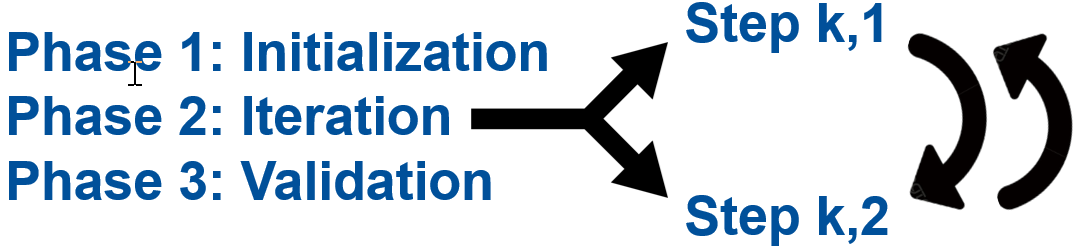
\includegraphics[width=0.6\columnwidth]{figures/AlgorithmPhases.png}
      \vspace{-0.2cm}\caption{ Structure of Optimization Algorithm}
      \label{AlgoPhases}
\end{figure} 

\vspace{-0.5cm}

\subsubsection{Initialization Phase} 

The objective of the first phase is essentially to provide an initial estimate for a state feedback gain matrix controller \textbf{K} that stabilizes the closed loop $\Dot{x}=(A+BK)x$. For this, the strategy taken is to fix the decision variables \textcolor{blue}{$\lambda$, M, H} present in (\ref{MainMatrixIneq}) in the following way:
\begin{equation}
\resizebox{0.15\textwidth}{!}{$
    \begin{gathered}
        \textcolor{blue}{\lambda} = \lambda = 0 \\
        \textcolor{blue}{M} = M_0 = \begin{pmatrix}
            C^{\circ}C\\
            {C^{\perp}}^T
        \end{pmatrix}\\
        \textcolor{blue}{H} = H_0 = J M_0^{-1} \\
        J = (-\mu-h)I,
    \end{gathered}$}
    \label{InitVariableFixing}
\end{equation} 

where, $h$ is a positive scalar and $-\mu$ is the maximum real part of the eigenvalues of A. The feasibility study that is conducted in the initialization phase is the following:

\vspace{-0.5cm}

\begin{equation}
\resizebox{0.45\textwidth}{!}{$
    \begin{gathered}
        \textcolor{blue}{P} \succ 0 \\
        He\left\{ \begin{bmatrix}
            0 & 0 & \textcolor{blue}{P}\\
            0 & 0 & 0\\
            \textcolor{blue}{P} & 0 & 0
        \end{bmatrix}\right\}
    \prec
    He\left\{\begin{bmatrix}
            I\\
            -M_0 \\
            -A
    \end{bmatrix}
    \textcolor{blue}{S_1} +
    \begin{bmatrix}
        0\\
        \textcolor{blue}{S_2}\\
        B\textcolor{blue}{Z}
    \end{bmatrix}
    \begin{bmatrix}
        0 & I & -H_0^T
    \end{bmatrix}\right\}
    \end{gathered}$}
    \label{InitMatrixIneq}
\end{equation} 

If (\ref{InitMatrixIneq}) is feasible for a combination of the decision variables \textcolor{blue}{$S_1,S_2$}, \textcolor{blue}{Z} and for the  Lyapunov certificate \textcolor{blue}{P}, then an initial guess of a stabilizing state feedback gain \textbf{K} is found, and one can pass to the iteration phase. On the other hand, if a solution is not found, the parameter \textbf{h} is increased by 1 and the initialization phase is executed again. This phase solves the (SI) and (SF) problems. The outputs of this phase are:

\begin{equation}
\resizebox{0.13\textwidth}{!}{$
    \begin{gathered}
        S_{1.0}=\textcolor{blue}{S_1}  \\
        \hat{K}_0 = -\textcolor{blue}{Z} \textcolor{blue}{S_2}^{-1} \\
        K = -\textcolor{blue}{Z} \textcolor{blue}{S_2}^{-1} M_0
    \end{gathered}$}
    \label{OutputsInit}
\end{equation}

\subsubsection{Iteration Phase - Step k,1}
This phase comprises two iterative steps. In the first step, the optimization variables $\pmb{\lambda}$ and \textbf{M} in \ref{MainMatrixIneq} previously fixed during initialization, are now treated as decision variables. To maintain convexity, the slack variable \textcolor{blue}{$S_1$} is set at the value $\pmb{S_{1,0}}$ determined in the initialization phase. Then, system (\ref{Iter1MatrixIneq}) is solved.

\vspace{-0.5cm}

\begin{equation}
\centering
\resizebox{0.48\textwidth}{!}{$
    \begin{gathered}
        \textcolor{blue}{P} \succ 0, \quad \begin{bmatrix}
            (1-\textcolor{blue}{\lambda})I & \textcolor{blue}{M^T}\\
            \textcolor{blue}{M} & I
        \end{bmatrix} \geq 0 ,\quad \textcolor{blue}{\lambda} \geq 0 \\
        He\left\{ \begin{bmatrix}
            0 & 0 & \textcolor{blue}{P}\\
            0 & 0 & 0\\
            \textcolor{blue}{P} & 0 & 0
        \end{bmatrix}\right\}
    \prec
    He\left\{\begin{bmatrix}
            I\\
            -\begin{pmatrix} \textcolor{blue}{\lambda}
            \begin{bmatrix}
                C\\
                0_{p-n,n}
            \end{bmatrix} +
            \textcolor{blue}{M}
            \end{pmatrix}\\
            -A
    \end{bmatrix}
    S_{1,k-1} +
    \begin{bmatrix}
         0\\
        -I\\
        B \hat{K}_{k-1}
    \end{bmatrix}
    \begin{bmatrix}
        0 & -\textcolor{blue}{S_2} & \textcolor{blue}{Y}^T
\end{bmatrix}\right\}
    \end{gathered}$}
    \label{Iter1MatrixIneq}
\end{equation}

In (\ref{Iter1MatrixIneq}), two matrix inequalities appear, in addition to the Lyapunov certificate inequality and the inequality (\ref{MainMatrixIneq}). These additional constraints, contribute towards achieving the objective of the iteration phase which is to find a solution for (\ref{MainMatrixIneq}) where the variables $\pmb{\lambda}$ and \textbf{M} converge to the values of 1 and 0, respectively, this being a mandatory requirement for meeting the main optimization goal. This is accomplished by setting the maximization of $\pmb{\lambda}$ as an objective in the optimization solver. The second matrix inequality works on constraining the norm of \textbf{M} and decreasing it to 0, as $\pmb{\lambda}$ increases to 1. The third inequality is merely a constraint on $\pmb{\lambda}$ to be positive.

If a solution is found for (\ref{Iter1MatrixIneq}) and if for this solution $1-\lambda$ is lower than a specific tolerance, this means that one can pass on to the third and last phase, namely the validation. The outputs for this phase are:

\begin{equation}
\resizebox{0.13\textwidth}{!}{$
    \begin{gathered}
        \lambda_k=\textcolor{blue}{\lambda}  \\
        M_k = \textcolor{blue}{M} \\
        H_k^T = \textcolor{blue}{S_2}^{-1} \textcolor{blue}{Y}^T
    \end{gathered}$}
    \label{OutputsIterStap2}
\end{equation}

If not, there is a second step in the iteration phase.

\subsubsection{Iteration Phase - Step k,2}
Step \textbf{k,2} is essentially an initialization step in disguise. Similar to the first phase, where \textcolor{blue}{$\lambda$, M} and \textcolor{blue}{H} were fixed as inputs to generate a stabilizing feedback gain \textbf{K}, the second step fixes the same decision variables with updated values from step \textbf{k,1}.

The optimization problem that needs to be solved in this phase is the following:

\vspace{-0.5cm}


\begin{equation}
\centering
\resizebox{0.48\textwidth}{!}{$
    \begin{gathered}
        \textcolor{blue}{P} \succ 0 \\
        He\left\{ \begin{bmatrix}
            0 & 0 & \textcolor{blue}{P}\\
            0 & 0 & 0\\
            \textcolor{blue}{P} & 0 & 0
        \end{bmatrix}\right\}
    \prec
    He\left\{\begin{bmatrix}
           I\\
                -\hat{M}(\textcolor{blue}{\alpha})\\
            -A
    \end{bmatrix}
    \textcolor{blue}{S_1} +
    \begin{bmatrix}
        0\\
        \textcolor{blue}{S_2}\\
        B\textcolor{blue}{Z}
    \end{bmatrix}
    \begin{bmatrix}
        0 & I & -H_k^T
    \end{bmatrix}\right\}
    \end{gathered}$}
    \label{Iter2MatrixIneq}
\end{equation}
\begin{equation}
\resizebox{0.38\textwidth}{!}{$
    \begin{gathered}
        \hat{M}(\textcolor{blue}{\alpha}) = \left((1+\textcolor{blue}{\alpha} (\lambda_k-1))
        \begin{bmatrix}
            C \\
            0_{p-n,n}
        \end{bmatrix}
        +
        \textcolor{blue}{\alpha} M_k\right)
    \end{gathered}$}
    \label{Artificiu2}
\end{equation}

In this step, a new term, M($\textcolor{blue}{\alpha}$) appears, dependent on a new decision variable $\textcolor{blue}{\alpha}$. The goal is to minimize \textcolor{blue}{$\alpha$} using the bisection method, converting the non-convex problem into a convex one. Ideally \textcolor{blue}{$\alpha$} converges to 0, signaling the end of this iteration phase and progression to the final validation phase. If $\alpha \approx 0$ within a certain tolerance, (\ref{Artificiu2}) simplifies to (\ref{Artificiu3}) and as a result, the values of the decision variables for the solution that has been found for (\ref{Iter2MatrixIneq}) that correspond to the step \textbf{k,2} are also values for which (\ref{MainMatrixIneq}) is solved when particularized for $\lambda = 1$ and M = 0. Finding a solution for (\ref{MainMatrixIneq}) with $\lambda = 1$ and M = 0, enables the computation of a stabilizing SOF controller.

\vspace{-0.5cm}


\begin{equation}
\resizebox{0.45\textwidth}{!}{$
    \begin{gathered}
        \hat{M}(\alpha) = \left((1+\alpha (\lambda_k-1))
        \begin{bmatrix}
            C \\
            0_{p-n,n}
        \end{bmatrix}
        + 
        \alpha M_k\right)
        \stackrel{\alpha \approx 0 }{=}
        \begin{bmatrix}
            C \\
            0_{p-n,n}
        \end{bmatrix}
    \end{gathered}$}
    \label{Artificiu3}
\end{equation}

If at step \textbf{k,2} $\alpha$ is not smaller than a fixed tolerance, the algorithm will start a new iteration step at \textbf{k,1}. The outputs of the current phase are:

\begin{equation}
\resizebox{0.14\textwidth}{!}{$
    \begin{gathered}
\alpha_k=\textcolor{blue}{\alpha}  \\
        \hat{K}_{k-1} = -\textcolor{blue}{Z} \textcolor{blue}{S_2}^{-1} \\
        S_{1,k} = \textcolor{blue}{S_1}
    \end{gathered}$}
    \label{OutputsIterStap1}
\end{equation}

\subsubsection{Validation Phase}

In cases where the iteration stage provides solutions for which $\pmb{\lambda}$ and \textbf{M} are exactly equal to 1 and 0, a validation phase is not required because a SOF controller can be computed directly. In practice, the algorithm exits the iteration phase with solutions for $\pmb{\lambda}$ and \textbf{M} close to 1 and 0, due to limitations of the optimization solvers and numerical accuracies. In these cases, the conditions for achieving the main optimization objective are not exactly met. As a result, a validation phase is necessary, where the problem to be solved is defined by (\ref{ValidMatrixIneq}) where the variables $\pmb{\lambda}$ and \textbf{M} are set to 1 and 0 and \textbf{H} is set to $H_k$ (obtained during the iteration phase). If a solution is found, the gain matrix \textbf{F} can be constructed with (\ref{GetF}) that is guaranteed to stabilize the closed loop (A+B\textbf{F}C). This last phase, provides the solution to the (OI) and (OF) goals. 

\vspace{-0.5cm}


\begin{equation}
\centering
\resizebox{0.48\textwidth}{!}{$
    \begin{gathered}
        \textcolor{blue}{P} \succ 0 \\
        He\left\{ \begin{bmatrix}
            0 & 0 & \textcolor{blue}{P}\\
            0 & 0 & 0\\
            \textcolor{blue}{P} & 0 & 0
        \end{bmatrix}\right\}
    \prec
    He\left\{\begin{bmatrix}
            I\\
                -\begin{bmatrix}
                    C \\
                    0_{p-n,n}
                \end{bmatrix}\\
            -A
    \end{bmatrix}
    \textcolor{blue}{S_1} +
    \begin{bmatrix}
        0\\
        \textcolor{blue}{S_2}\\
        B\textcolor{blue}{Z}
    \end{bmatrix}
    \begin{bmatrix}
        0 & I & -H^T
    \end{bmatrix}\right\}
    \end{gathered}$}
    \label{ValidMatrixIneq}
\end{equation}


\subsection{Plant Augmentation and Control Architecture}
\label{3b}

The control architecture for the DarkO drone is designed to stabilize it during hovering, both with and without external disturbances. For example, to counteract a headwind affecting linear velocity along the $x_{[b]}$ and $z_{[b]}$ axes and generating a moment about the $y_{[b]}$ axis, the control scheme uses the ailerons and propellers symmetrically to generate a compensatory moment and force. Integral action is employed to counteract the force along the $z_{[b]}$ axis, ensuring asymptotic convergence to the desired force using two integrators, one for the motors and one for the elevons. Other common control methods for this drone configuration include PID scheduling, decoupled speed and attitude controllers, and nonlinear controllers with command allocation. However, none of these approaches directly address wind effects.

The synthesis of a SOF controller for the  augmented DarkO dynamics takes its inspiration from \cite{SYRMOS1997125} where it is shown that a dynamic output compensator of order $q \leq n$ (n-plant order), can be converted to a static output feedback through state-space augmentation. In our case, dynamic terms such as integrators and filters are added to the plant dynamics, resulting in an augmented state-space for which a static feedback law comprised of a pre-compensator static gain matrix will be synthesised. The implemented architecture, presented in Fig. \ref{Plant Augmentation}, is a reformulation of the control law presented in \cite{SANSOUACA}. It is composed of the linearized DarkO drone dynamic block, the saturation block for the two propellers and the two elevons that introduces limitations for the angular speed and angular rate of the electrical motors as well as angular deflection and angular rate for the control surfaces. The introduction of the actuator dynamics is subject for future studies. The output selection matrix eliminates the measurement of the pitch angle state, $\boldsymbol\theta$.

\vspace{-0.1cm}

\begin{figure}[hbt]
    \centering
    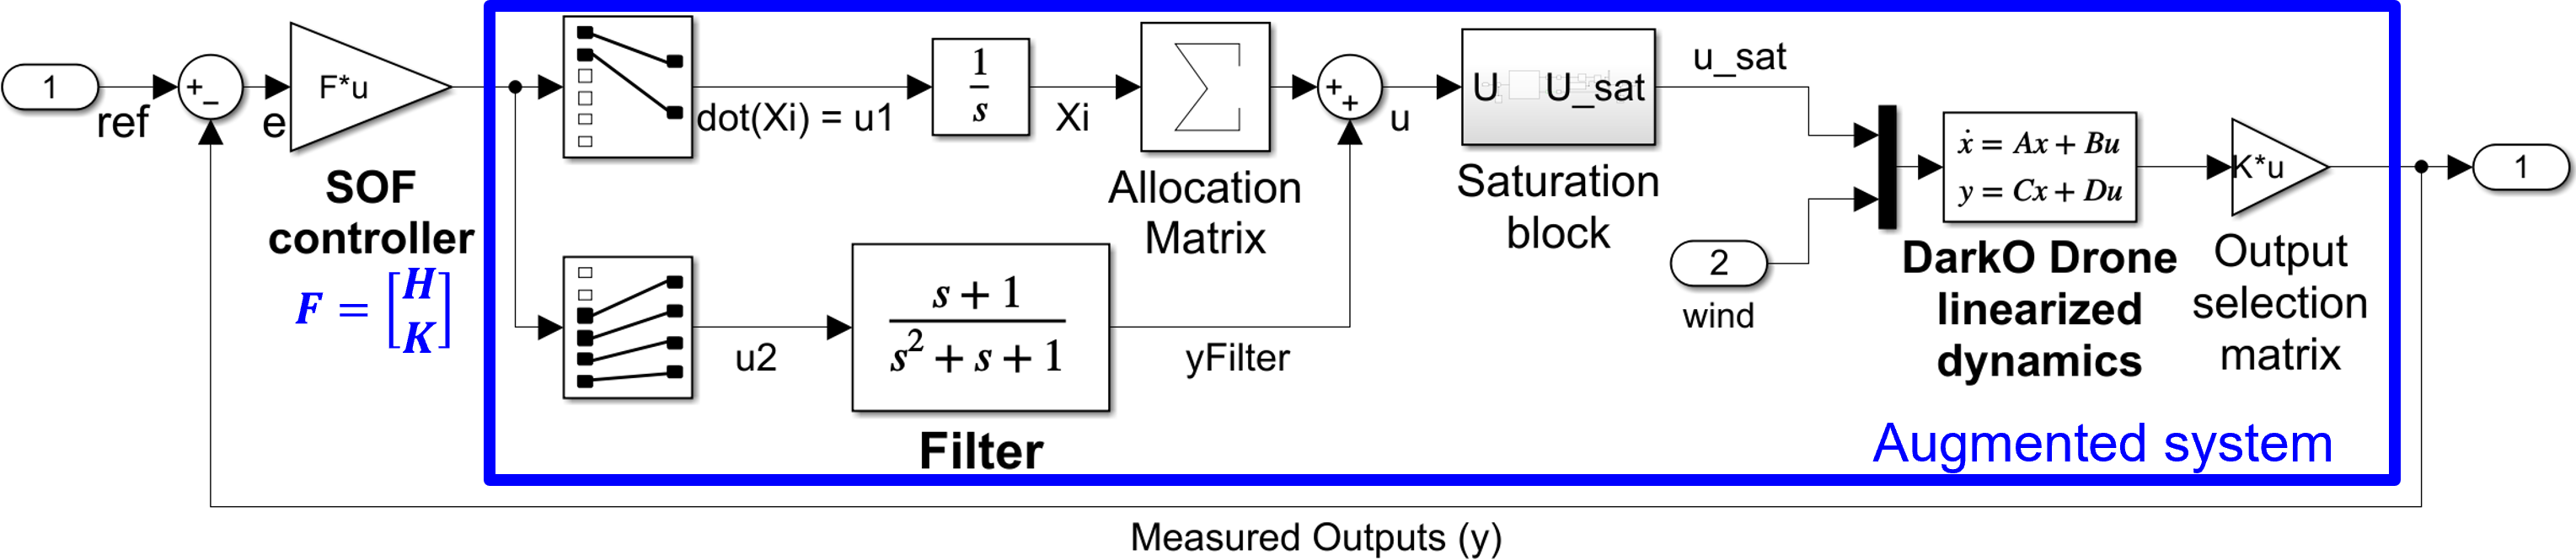
\includegraphics[width=0.9\columnwidth]{figures/AugWindFinal.png}
    \vspace{-0.3cm}\caption{Plant Augmentation}
    \label{Plant Augmentation}
\end{figure}

For control design, a PI-like controller structure is employed to minimize static error and enhance rejection of external disturbances. This is done by adding pre-compensator filters at the input of the system, based on the open-loop shaping methodology \cite{McFarlane1992} where an integrator is added to ensure performance (high gain) at low frequency, which corresponds to the tracking specification, and a second-order filter is added to ensure that the controller is strictly proper and to be robust with respect to neglected dynamics thanks to a roll-off behaviour. The filter's cutoff frequency is set at approximately 5 Hz to align with closed-loop dynamics and reject white noise in measured signals. For limiting the number of integrators to 2 (one that generates the integrative command for the two propellers and the other one for the two elevons) the outputs of the integrator block are doubled by an allocation matrix $ \sum $. Implementing a second order filter comes with the extra benefit of avoiding a direct feed-forward term, that may amplify unwanted sensor noise. The SOF matrix \textbf{F} comprises the gain matrices \textbf{H} and \textbf{K} for the integrative and proportional action, respectively. The equations and the state-space representation of the augmented plant are found in (\ref{AugEq1}) and (\ref{AugEq2}).

\vspace{-0.5cm}


\begin{equation}
\centering
\resizebox{0.44\textwidth}{!}{$
    \begin{gathered}
        \dot{x}_i = u_1 \\
        u = \sum x_i + y_{filter} = \sum x_i + Filter \cdot u_2 \\
        \dot{x} = Ax + Bu = Ax + B(\sum x_i + y_{filter}) = Ax + B\sum x_i + B C x_{filter} \\
        \sum =
        \begin{bmatrix}
            1 & 0 \\ 1 & 0 \\ 0 & 1 \\ 0 & 1   
        \end{bmatrix} \quad \quad
        \begin{bmatrix}
            u_1 \\ u_2   
        \end{bmatrix}
        = F e = F \left(\begin{bmatrix}ref \\ \mathbb{0}_{8\times 1} \end{bmatrix}-y\right)  
    \end{gathered}$}
    \label{AugEq1}
\end{equation}
\begin{equation}
\centering
\resizebox{0.44\textwidth}{!}{$
    \begin{gathered}
        \begin{pmatrix}
            \Dot{x} \\ \Dot{x_c} \\ \Dot{x}_{filter}
        \end{pmatrix} =
        \begin{bmatrix}
            A & B \sum & B C_{filter} \\
            0 & 0 & 0 \\
            0 & 0 & A_{filter} 
        \end{bmatrix}
        \begin{pmatrix}
            x \\ x_c \\ x_{filter}
        \end{pmatrix}
        +
        \begin{bmatrix}
            0 & 0 \\ 1 & 0 \\ 0 & B_{filter}
        \end{bmatrix}
        \begin{bmatrix}
            u_1 \\ u_2
        \end{bmatrix}  \\
        y = \begin{bmatrix}
            C & 0 & 0
        \end{bmatrix}
        \begin{pmatrix}
            x \\ x_c \\ x_{filter}
        \end{pmatrix}
    \end{gathered}$}
    \label{AugEq2}
\end{equation}

Where \textit{$x_i$} $\in \mathbb{R}^{2}$ - integrative states, \textit{$x_f$} $\in \mathbb{R}^{4}$ - filter states, \textit{r} $\in \mathbb{R}^{3}$ - reference signal, \textit{y} $\in \mathbb{R}^{11}$ - measured states and \textit{u} $\in \mathbb{R}^{4}$ - plant input.

\section{Results}

\subsection{Simulation Results}

The approach from section  \ref{3a} was applied to the augmented system from section \ref{3b}, focusing on the linearized dynamics for a wind speed of 0 (hovering scenario). This resulted in four stabilizing controllers for h=12,13,14, and 15, with h varying between 1 and 40. Multiple iterations with different h values, serving as various initialization points for the optimization algorithm, are necessary to enhance the likelihood of convergence.

Figure \ref{HKStepRes_a} shows the closed-loop temporal response of the four controllers, with reference steps for the x-axis at 5s, y-axis at 90s, and z-axis at 40s. All controllers effectively stabilize the closed-loop dynamics and track position references on the XYZ axes. The response is slow on the X and Z axes and fast on the Y axis. Notably, a position step on one axis does not cause significant offset or change on the other two axes, indicating strong decoupling between the XYZ position states. Additionally, the actuators were never saturated.

\begin{figure}[hbt]
    \centering
   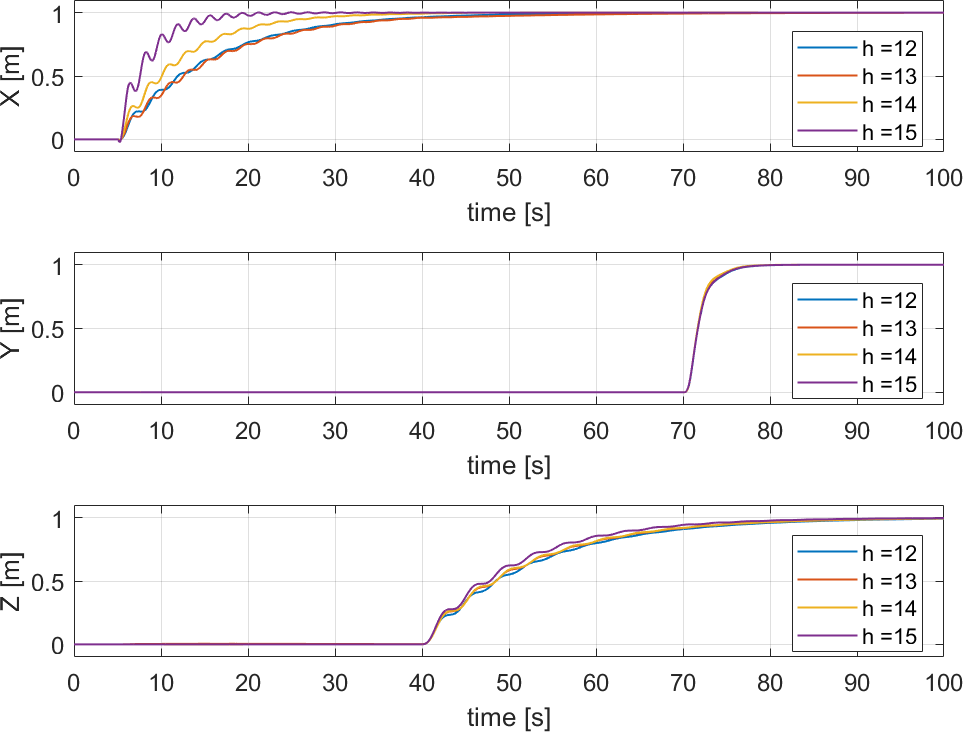
\includegraphics[width=0.9\columnwidth]{figures/stepResponse.png}
    \vspace{-0.3cm}\caption{Closed-Loop response of SOF controllers - Linear Dynamics}
    \label{HKStepRes_a}
\end{figure}

The first subplot of Fig. \ref{thetanowind} shows that the state $\pmb{\theta}$ experiences increasing oscillations as h increases. While the pitch angle $\pmb{\theta}$ is not directly controlled, it naturally converges to 0 as the other states stabilize, indicating hovering flight without wind. The second subplot demonstrates that for dynamics linearized around a specific wind speed, $\pmb{\theta}$ converges to a non-zero value, compensating for external disturbances.

\begin{figure}[hbt]
    \centering
    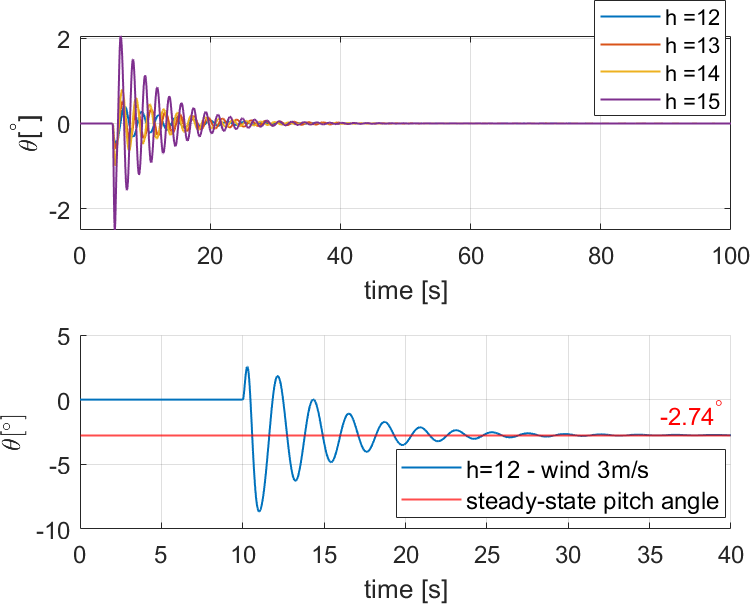
\includegraphics[width=0.9\columnwidth]{figures/windThetafinalhopeCrop.png}
    \vspace{-0.3cm}\caption{Closed-Loop temporal response - theta state}
    \label{thetanowind}
\end{figure}


% Figures \ref{Input_Sensitivity} and \ref{Output_Sensitivity} show that for every trimming point of the linearized dynamics, the algorithm was able to provide stabilizing SOF controllers. In terms of robustness, the $H_\infty$ norm of the input sensitivity for the synthesized controllers is under 10 dB while for the output sensitivity,
% it is over 40 dB.

% \begin{figure}[hbt]
%     \centering
%     \includegraphics[width=0.9\columnwidth]{Figures/Input_Sensitivity.eps}
%     \vspace{-0.3cm}\caption{Input Sensitivity}
%     \label{Input_Sensitivity}
% \end{figure}
% \begin{figure}[hbt]
%     \centering
%     \includegraphics[width=0.9\columnwidth]{Figures/Output_Sensitivity.eps}
%     \vspace{-0.3cm}\caption{Output Sensitivity}
%     \label{Output_Sensitivity}
% \end{figure} 


For analysis purposes, Eq. \ref{Kstructure1} and \ref{Kstructure2} present the gains of the synthesized controller \textbf{F} (block illustrated in \ref{Plant Augmentation}) comprising the matrix gains \textbf{H} and \textbf{K} for h=12 and linearized dynamics at 0 wind speed. By taking a more attentive look at the gain matrix \textbf{K} that outputs 4 command signals used for the asymmetric or symmetric control of the drone actuators, one can observe that for the $1^{st}$ and $2^{nd}$ rows (that generate a demand of thrust of the two propellers) as well as for $3^{rd}$ and $4^{th}$ rows (that generate a demand for a deflection angle for the two elevons) are either nearly equal or opposite, with few exceptions. This pattern emerged naturally from the optimization process without any constraints, reflecting an intuitive and coherent alignment with the drone's dynamics.

\begin{equation}\label{Kstructure1}
\scalebox{0.5}{$H=
\!\begin{aligned}
&
\left[\begin{matrix}
  3.5e-06 & -3.0e-07 &  1.5e-02 & -6.9e-06 & -7.4e-06 &  4.4e-01 \\
  -2.0e-02 & -7.5e-06 &  1.6e-05 & -2.0e-01 &  4.4e-05 & -1.1e-04
\end{matrix}\right.\\
&\qquad\qquad
\left.\begin{matrix}
  {}1.8e-04 &  1.1e-04 & -8.4e-05 & -8.6e-05 & -2.3e-04\\
  {}-9.2e-05 & -9.1e-05 &  7.4e-06 &  7.6e-01 & -3.9e-05
\end{matrix}\right]
\end{aligned}$}
\end{equation}
%\vspace{-0.5cm}
 \begin{equation}\label{Kstructure2}
\scalebox{0.5}{$K=
\!\begin{aligned}
&
\left[\begin{matrix}
  7.6e-03 & -2.0e+01 &  9.9e+00 &  3.1e-02 & -4.5e+01 &  8.2e+01 \\
  5.4e-03 &  2.0e+01 &  9.9e+00 &  8.8e-03 &  4.5e+01 &  8.2e+01 \\
  -4.2e+00 & -3.2e-01 &  8.7e-03 & -4.5e+01 & -4.4e-01 & -3.1e-02 \\
  -4.2e+00 &  3.2e-01 &  4.8e-03 & -4.5e+01 &  4.3e-01 &  3.3e-02
\end{matrix}\right.\\
&\qquad\qquad
\left.\begin{matrix}
  {}-3.1e+02 & -3.1e+02 &  6.4e-01 &  3.0e-03 & -1.0e+02\\
  {}3.1e+02 &  3.1e+02 & -6.5e-01 & -1.9e-03 &  1.0e+02 \\
  {}-1.2e+01 &  1.6e+00 & -3.1e+01 &  3.9e+01 & -1.6e+00 \\
  {}1.2e+01 & -1.7e+00 &  3.1e+01 &  3.9e+01 &  1.6e+00
\end{matrix}\right]
\end{aligned}$}
\end{equation}

%For a better understanding, one can take the case where the drone's error or offset between the reference and actual position on X is positive. By examining the first column of the K matrix, it can be said that the gains for the propellers ($1^{st}$ and $2^{nd}$ rows) are extremely low meaning that the position error on X will not force a variation of the propeller angular speed, whereas in the case of the  $3^{rd}$ and $4^{th}$ row, both gains are negative which will generate a symmetrical command to lower the elevons in order to correct the error. In the case of a positive position error on Y axis, the gains for the propellers and elevons are opposite which will generate asymmetric commands while for a positive error on Z axis the gains for the propellers are high and positive whereas the gains for the elevons are low. This will be translated into an increase of propeller speed to reduce the error on Z axis and a small variation of the elevons angle to keep a vertical trajectory.


\subsection{Experimental Results}
For experimental validation, the designed controllers and architecture were tested on the real DarkO drone model built at ENAC Fig. \ref{DarkO1}. DarkO is assembled from multiple 3D printed Onyx parts (a robust material comprising omnidirectional carbon fibres). Flight tests took place in ENAC's volière, equipped with an Optitrack motion capture system providing position and attitude data at 40Hz, eliminating the need for a GPS sensor. Speed is obtained by a finite difference between the position. Data fusion algorithms, including Invariant Filters \cite{condomines2013,Condomines2014}, combined data from Optitrack (position, speed and attitude) and the DarkO drone's IMU unit for improved state estimation. This estimate is used to create the output vector $y$ used by the control law \eqref{AugEq1}. Given the architecture of the control loop, the estimation must be of very high quality with the lowest possible delay.
Paparazzi UAV open-source software and hardware packages were utilized \cite{hattenberger2014} and the modular nature of Paparazi permit to use the existing implementation of the invariant filter to estimate the DarkO state vector and to add a stabilisation module based on the control law described above (see \ref{3b}). This software is embedded in an autopilot designed and manufactured at Enac, an Apogee autopilot board\footnote{Product data sheet - \url{https://wiki.paparazziuav.org/wiki/Apogee/v1.00}} for processing. The autopilot board sampled command and control laws at 500Hz, generating appropriate control commands to achieve the desired flight manoeuvres and store all the data for posterior analysis.
\begin{figure}[ht]
    \centering
    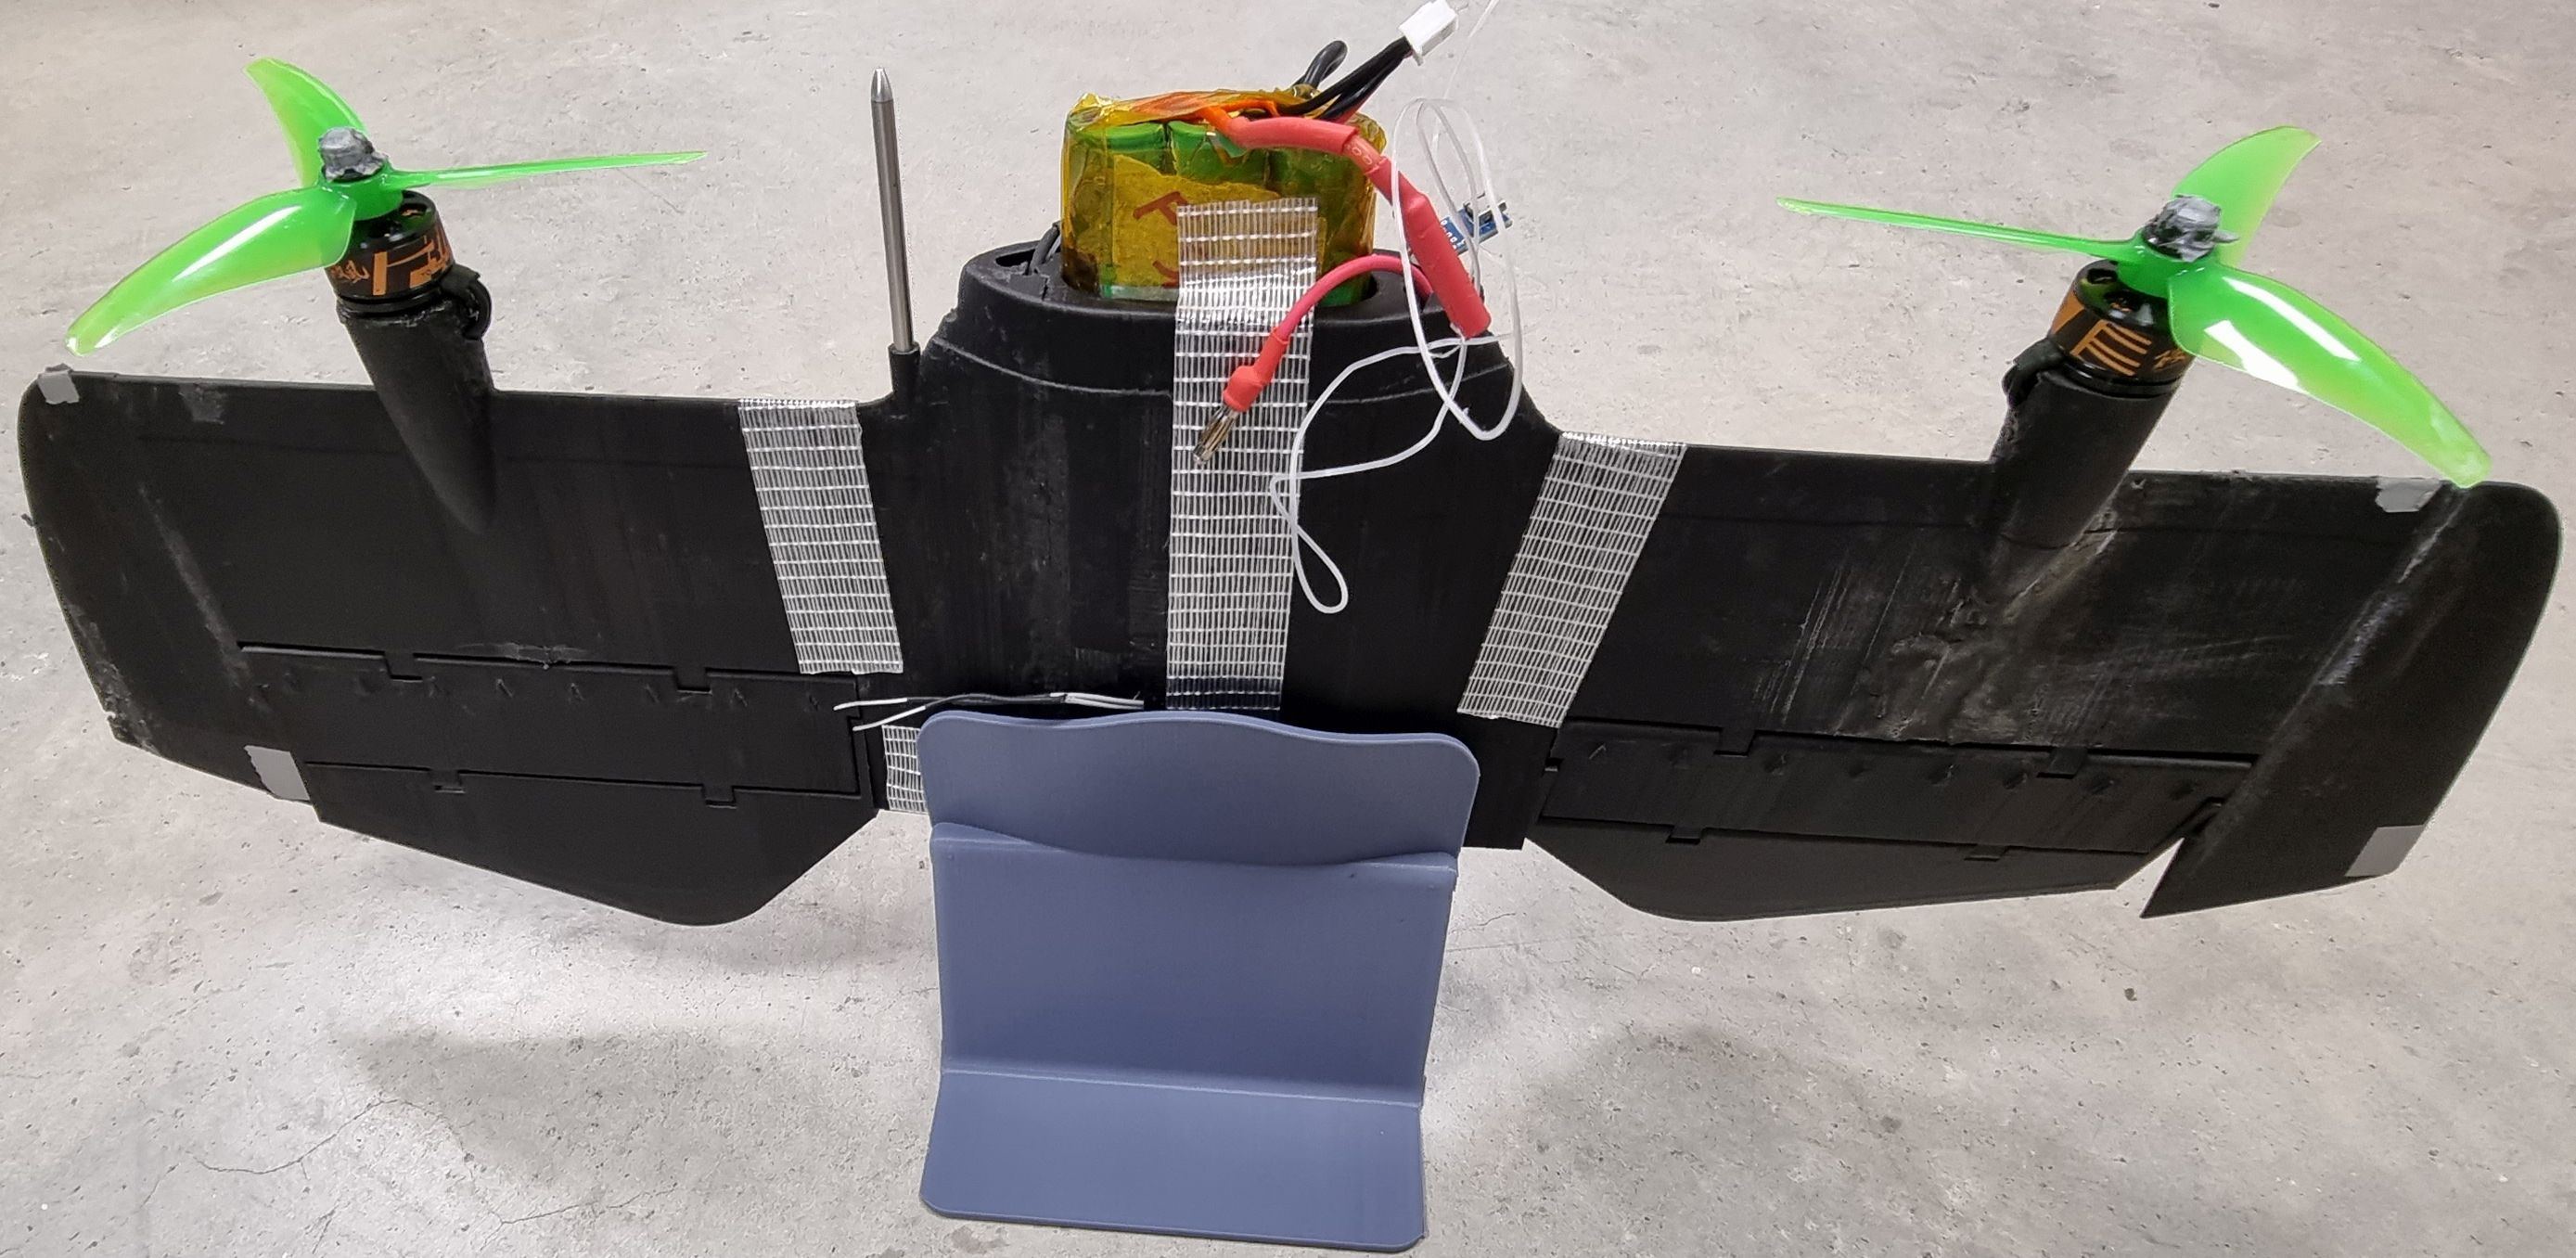
\includegraphics[width=0.8\columnwidth]{figures/DarkOModelfinal.jpg}
   \vspace{-0.2cm}\caption{DarkO Drone experimental model}
    \label{DarkO1}
\end{figure}
\begin{figure}[ht]
    \centering
    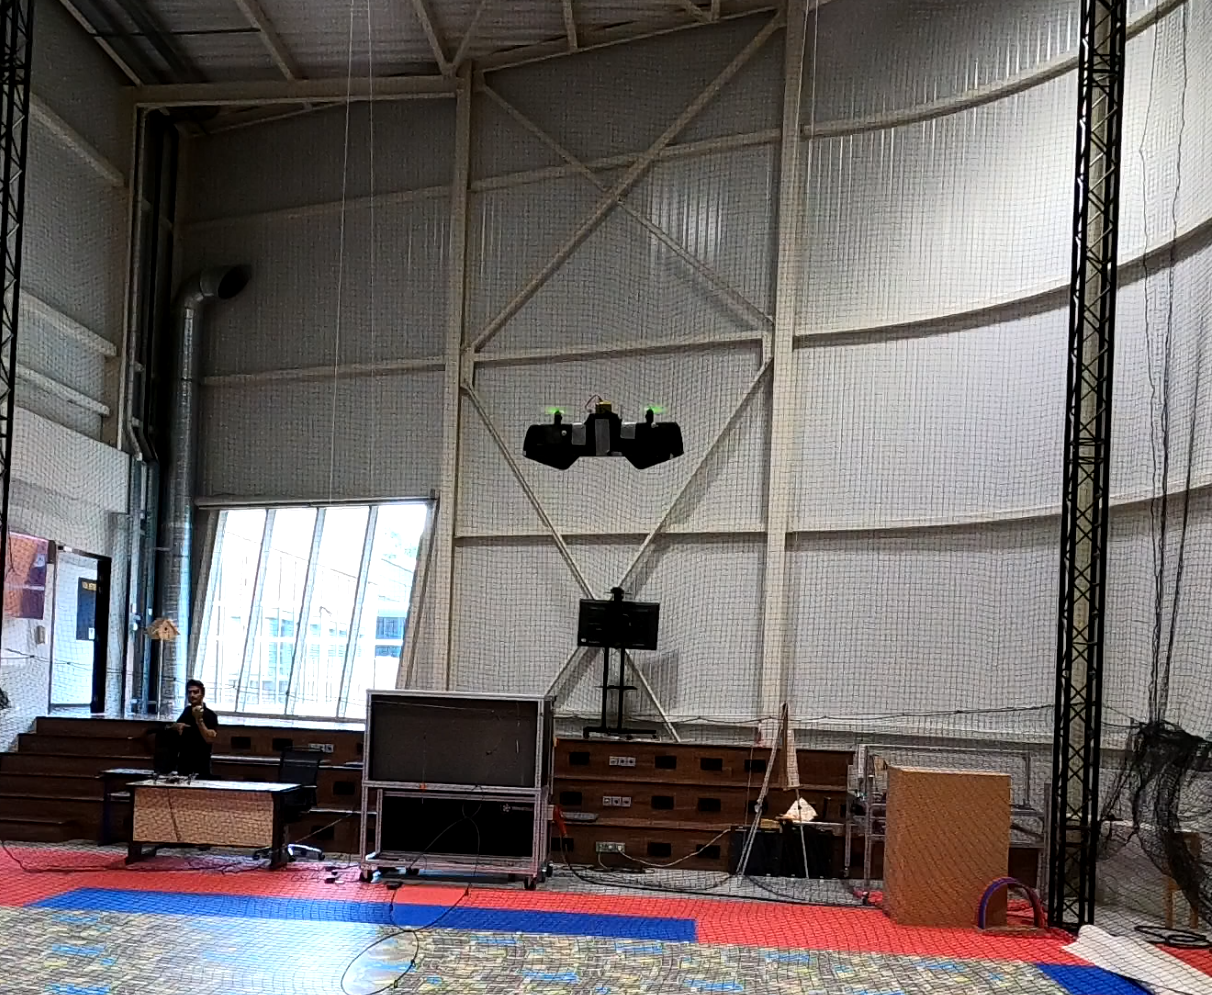
\includegraphics[width=0.8\columnwidth]{figures/DarkOFlighthope.png}
    \vspace{-0.2cm}\caption{DarkO drone during an experimental flight test}
    \label{DarkO2}
\end{figure}

The following experimental flight tests mark the first and only successful simulations in ENAC's volière where controllers  relying exclusively on model-based synthesis methods were used to control a convertible drone. Prior flights for this drone type utilized combined model– and sensor–based control designs like INDI algorithms. Each flight starts with the drone taking off and stabilizing at a reference position using an INDI controller. After reaching the desired hovering location, the INDI controller is replaced with the model-based controller. Figure \ref{SYSTUNE and Dabbene Flight Test Command} shows the flight test results of one of the four synthesized controllers for the designed control architecture. Figure \ref{DarkO2} depicts the DarkO drone during its test flight. All four controllers were tested and validated on the real system, demonstrating stable performance and accurate position tracking on all three axes.


\begin{figure}[h]
    \centering
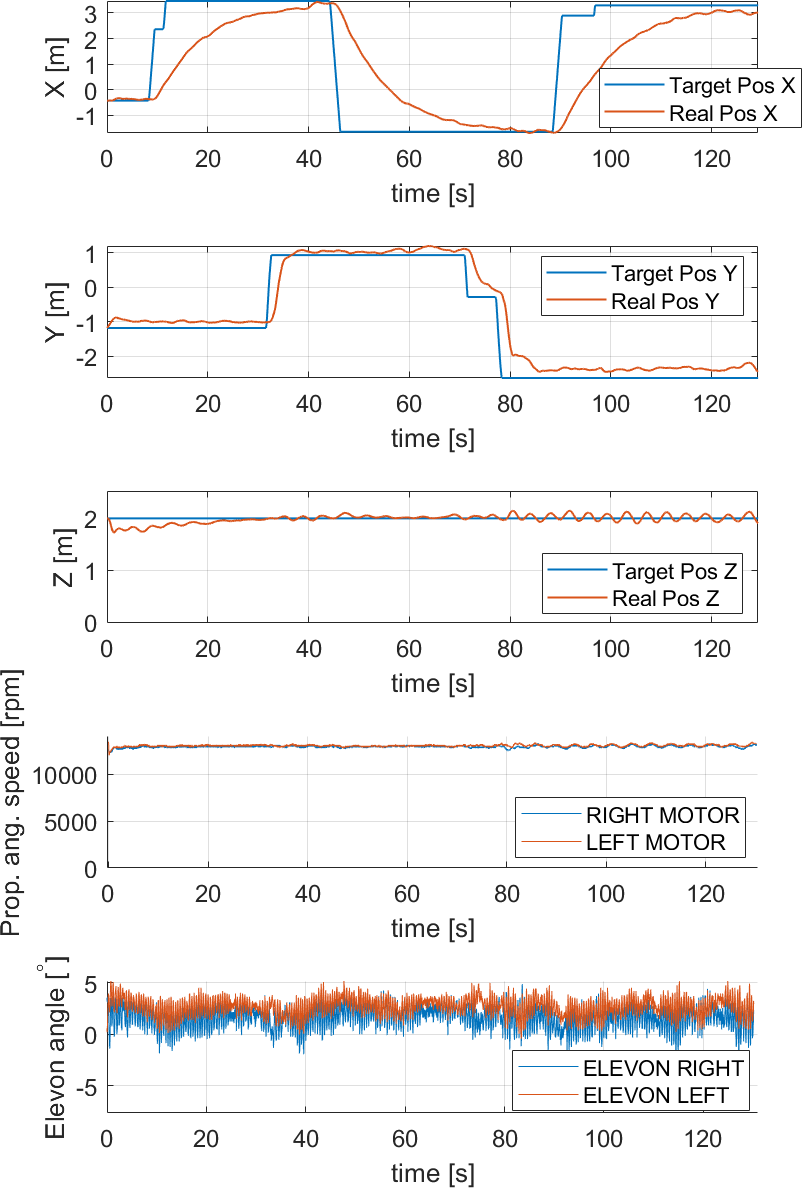
\includegraphics[width=1\columnwidth]{figures/realflight_z_adjust_x_adjust_final_HopeCrop.png}
   \vspace{-0.5cm}\caption{Flight Test, Closed-Loop Response and Command Input, h = 12}
    \label{SYSTUNE and Dabbene Flight Test Command}
\end{figure}

As it was also observed in the simulations, on the X and Z axes, the time response is relatively high whereas on the Y axis, the time response is drastically quicker, due to the strong differential actuation on this axis backed up by the fast actuator dynamics. On the Z axis, the switch from the INDI controller to the synthesised controller, results in a relatively important vertical descent of the drone. As a consequence, further tuning and modeling needs to be performed in order to correct the state and command input initialization values corresponding to the equilibrium point. The dynamic of the drone on Z is characterized by small oscillations around the reference position, that can also be observed in the command signal of the angular speeds of the propellers, illustrated in  Fig. \ref{SYSTUNE and Dabbene Flight Test Command}. These reduced oscillations are due to the actuator dynamics not being considered in the control law. This problematic will be studied in the future, particularly with the use of a motor speed controller (see AM32-MultiRotor-ESC-firmware~\footnote{\url{https://github.com/FlorianSan/AM32-MultiRotor-ESC-firmware}}). It's worth noting that the optimization algorithm's primary objective is to achieve closed-loop stabilization, disregarding performance or robustness criteria. During experimental flights, the controller did not saturate the actuators (see Fig. \ref{SYSTUNE and Dabbene Flight Test Command}).


\section{Conclusion du Chapitre \ref{chap:LMI}}

A convex optimization algorithm, utilizing the LMI framework and Lyapunov’s stability theory, was employed to synthesize SOF controllers for the DarkO convertible drone model. This model-based synthesis technique effectively stabilized the closed-loop dynamics of the augmented plant, ensuring satisfactory temporal response and reference tracking without actuator saturation. Despite incomplete modeling of nonlinear phenomena, the controllers demonstrated robustness during initial experimental demonstrations on the DarkO drone model. With the designed SOF controller matrices and command law structure, successful experimental flights were conducted for hovering and trajectory tracking. This outcome serves as a solid proof of concept for the developed control law in terms of performance and robustness.